%%% Local Variables:
%%% TeX-master: "slides"
%%% End:

% \section{Model}


% \begin{frame}{Model Background}
%   \begin{center}
%     \scalebox{2}{
%   \begin{tikzpicture}

%     \node<1> at (10mm, 15mm){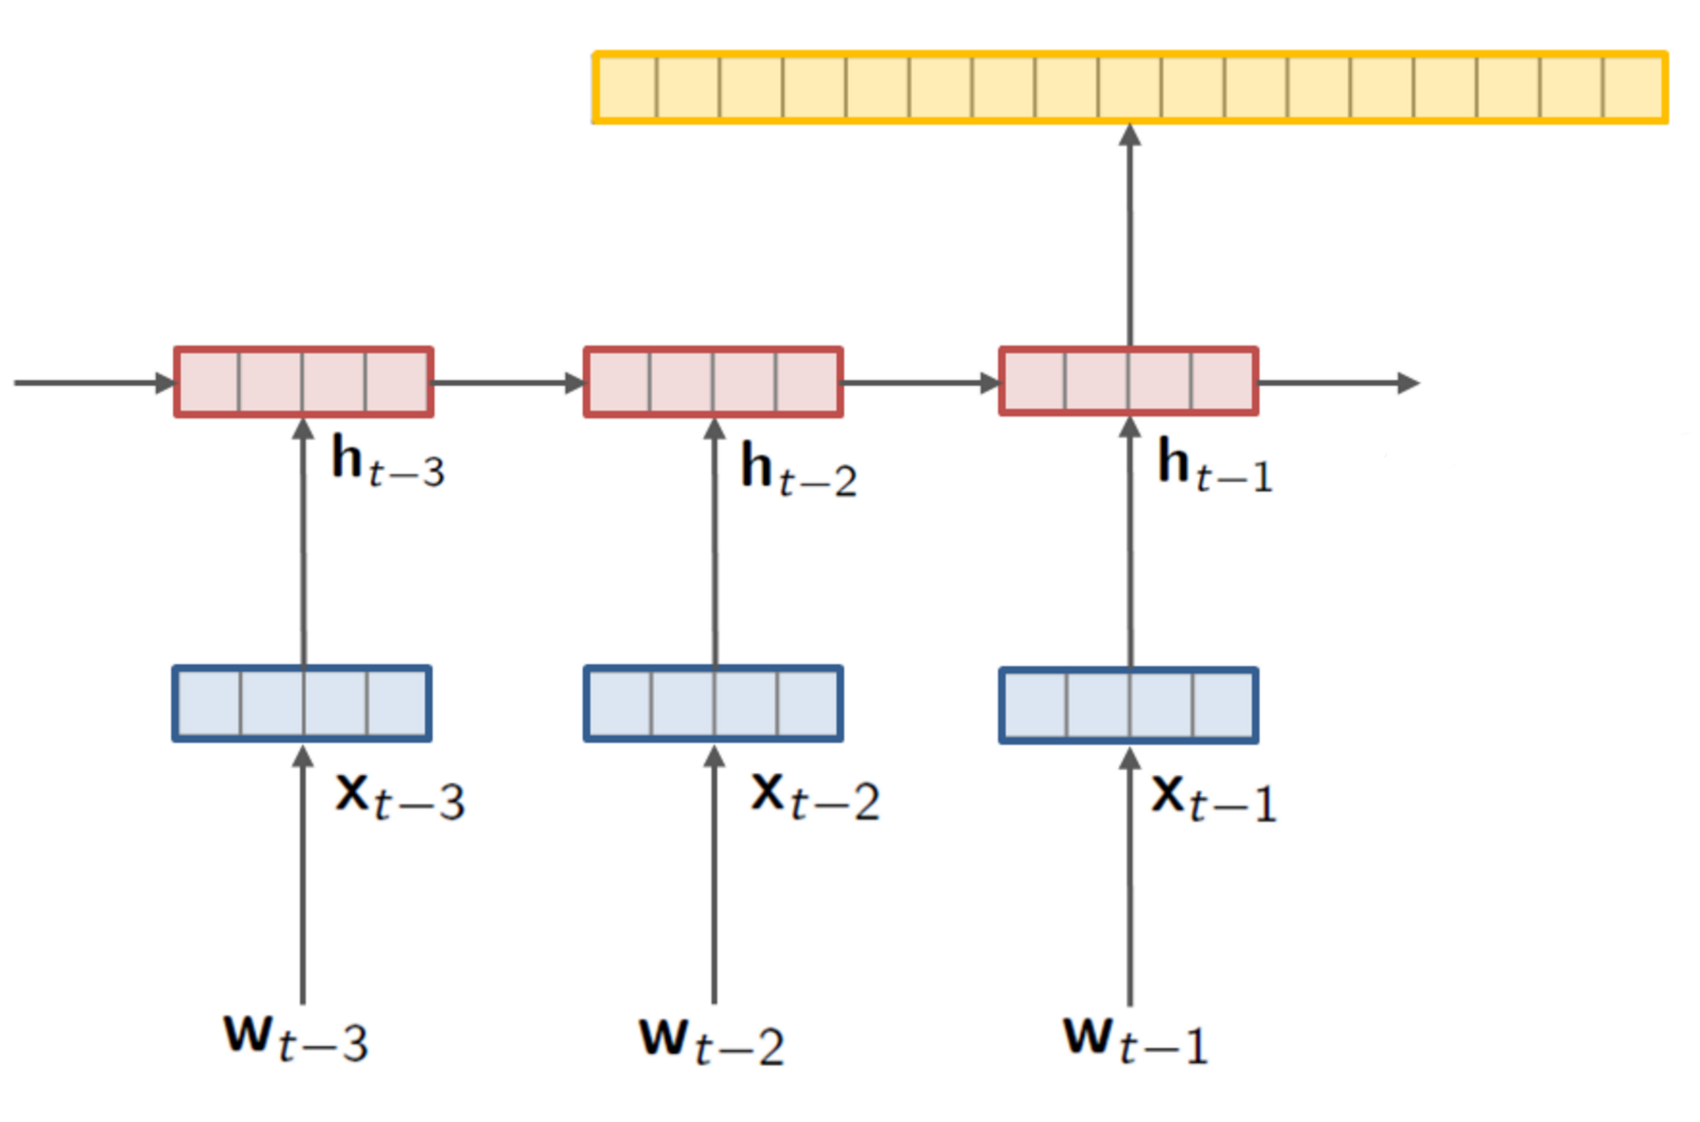
\includegraphics[width=3cm]{rnnlm6}};
%     \node[draw,  fill=yellow, thick, rounded corners, scale=0.5] (ana) at (-15mm, 15mm) {Analysis};
%     \node[draw,  thick, rounded corners,scale=0.5] (meth) at (0mm, 30mm) {\ Methods\phantom{p}};
%     \node[draw,  thick, rounded corners,scale=0.5] (app) at (25mm, 30mm) {Applications};b
%     \node[draw, thick, rounded corners, scale=0.5] (und) at (35mm, 15mm) {Understanding};
%     \node[draw, thick, rounded corners, scale=0.5] (dep) at (25mm, 0mm){Deployment};

%     \node[draw, fill=yellow, thick, rounded corners,scale=0.5] (imp) at (0, 0) {Implementation};

%     \draw (ana) -- (meth) --(app) -- (und) -- (dep) -- (imp) -- (ana);

%   \end{tikzpicture}
% }
%   \end{center}


% \end{frame}

% \begin{frame}{Machine Learning for Text Generation}
%     \[ y^*_{1:T} = \argmax_{y_{\tikzmark{opt}1:T}} \alert{f}(y_{1:T}; \tikzmark{input}x, \tikzmark{nn}\alert{\theta}) \]

% % \begin{tikzpicture}[
% %   remember picture,
% %   overlay]

% % \node (ptdex) [below left=  of {pic cs:pd}] {Output};
% % \node (ptdexa) [below right =  of {pic cs:nn}] {Neural Network};
% % \node (ptdexb) [below = of {pic cs:opt}] {Optimization};
% % \node (ptdexc) [below = of {pic cs:input}] {Input};
% % \draw[->] (ptdex.north) -- ({pic cs:pd});
% % \draw[->] (ptdexa.north) -- ({pic cs:nn});
% % \draw[->] (ptdexb.north) -- ({pic cs:opt});
% % \draw[->] (ptdexc.north) -- ({pic cs:input});
% % \end{tikzpicture}

%   \begin{itemize}

%   \item Input {$x_{1:S}$},  \textit{what to talk about}
%     \air

%   \item Output text {$y^*_{1:T}$}, \textit{how to say it}
%     \air

%   \item Model \alert{$f(.; \theta)$}, learned from data
%   \end{itemize}
% \end{frame}

\begin{frame}{Encoder-Decoder}{\large $f_{\theta}(y_{1:T}, x_{1:S})$}

  \vspace{-0.25cm}

  \begin{center}
    \multiinclude[format=png,start=1,graphics={height=0.85\textheight, trim=0.5cm 0.5cm 0.5cm 0.5cm, clip}]{nmt-noattn}
  \end{center}
\end{frame}


\begin{frame}{Encoder-Decoder}
  \textcolor{blue}{Encoder}:
  \[{\mathbf{h}^{x}_s \gets \RNN(\mathbf{h}^{x}_{s-1}, x_s; \theta)} \]


  \textcolor{orange}{Context}:
  \[ {\mathbf{c}} = \mathbf{h}^{x}_S \]
  \begin{center}
    \includegraphics<1>[height=0.6\textheight, trim=0.5cm 0.5cm 0.5cm
    0.5cm, clip]{nmt-noattn-2}
  \end{center}
  \pause
  \vspace{-0.5cm}

  \textcolor{red}{Decoder}:
  \[{\mathbf{h}_t \gets \RNN(\mathbf{h}_{t-1}, y_t; \theta)} \]

  Next Word Probability:
  \[ p(y_{t}\  |\  y_{1:t-1}, x) = \softmax( \mathbf{W} [\mathbf{h}_{t-1}; \mathbf{c}]) \]

  \pause

  Generation Score:
  \[  f_{\theta}(y_{1:T}, x) =   \sum_{t=1}^T \log p(y_{t}\  |\  y_{1:t-1}, x; \theta) \]

\end{frame}

\begin{frame}{Scoring Model Example }
  \textcolor{red}{Decoder}:
  \[{\mathbf{h}_t \gets \RNN(\mathbf{h}_{t-1}, y_t; \theta)} \]

  \air
 
  \textbf{Language} : Well-balanced parentheses (Dyck-1 Language) with  nesting-levels,
  \begin{itemize}
  \item Vocabulary: ( ) 0 1 2 3 4
  \item Example Good String: 0 ( ( 2 ) ( ( ( 4 4 4 ) 3 ) $\ldots$
  \item Example Bad String: 0 ) ( 3 ) ) ( (   $\ldots$
  \end{itemize}
  % Proxy Question: What does $\mathbf{h}_t$ look like over time?
\end{frame}

\begin{frame}{LSTMVis - Parenthesis Language}
  \research{\citet{Strobelt2016} w/ IBM}
  \vspace{-0.25cm}

  \begin{center}
    \movie[width=\textwidth, height=0.85\textheight, poster, showcontrols]{Temporary}{videos/lstmvis1.mp4}
  \end{center}
\end{frame}


% \begin{frame}{What can the decoder learn to say?}
%   \textcolor{red}{Decoder}:
%   \[{\mathbf{h}_t \gets \RNN(\mathbf{h}_{t-1}, y_t)} \]

%   \pause

%   \air

%   \textbf{Harder Example}:
%   Natural language outputs with complex syntax.


%   % Proxy Question: What does $\mathbf{h}_t$ look like over time?
% \end{frame}

\begin{frame}{LSTMVis - Parenthesis Language}
  \research{\citet{Strobelt2016} w/ IBM}
  \vspace{-0.25cm}

  \begin{center}
    \movie[width=\textwidth, height=0.85\textheight, poster, showcontrols]{Temporary}{videos/lstmvis1.mp4}
  \end{center}
\end{frame}


\begin{frame}{LSTMVis - Natural Language}
  \research{\citet{Strobelt2016} w/ IBM}
  \vspace{-0.25cm}


  \begin{center}
    \movie[width=\textwidth, height=0.85\textheight, poster, showcontrols]{Temporary}{videos/lstmvis2.mp4}
  \end{center}
\end{frame}


\begin{frame}
  \begin{center}
    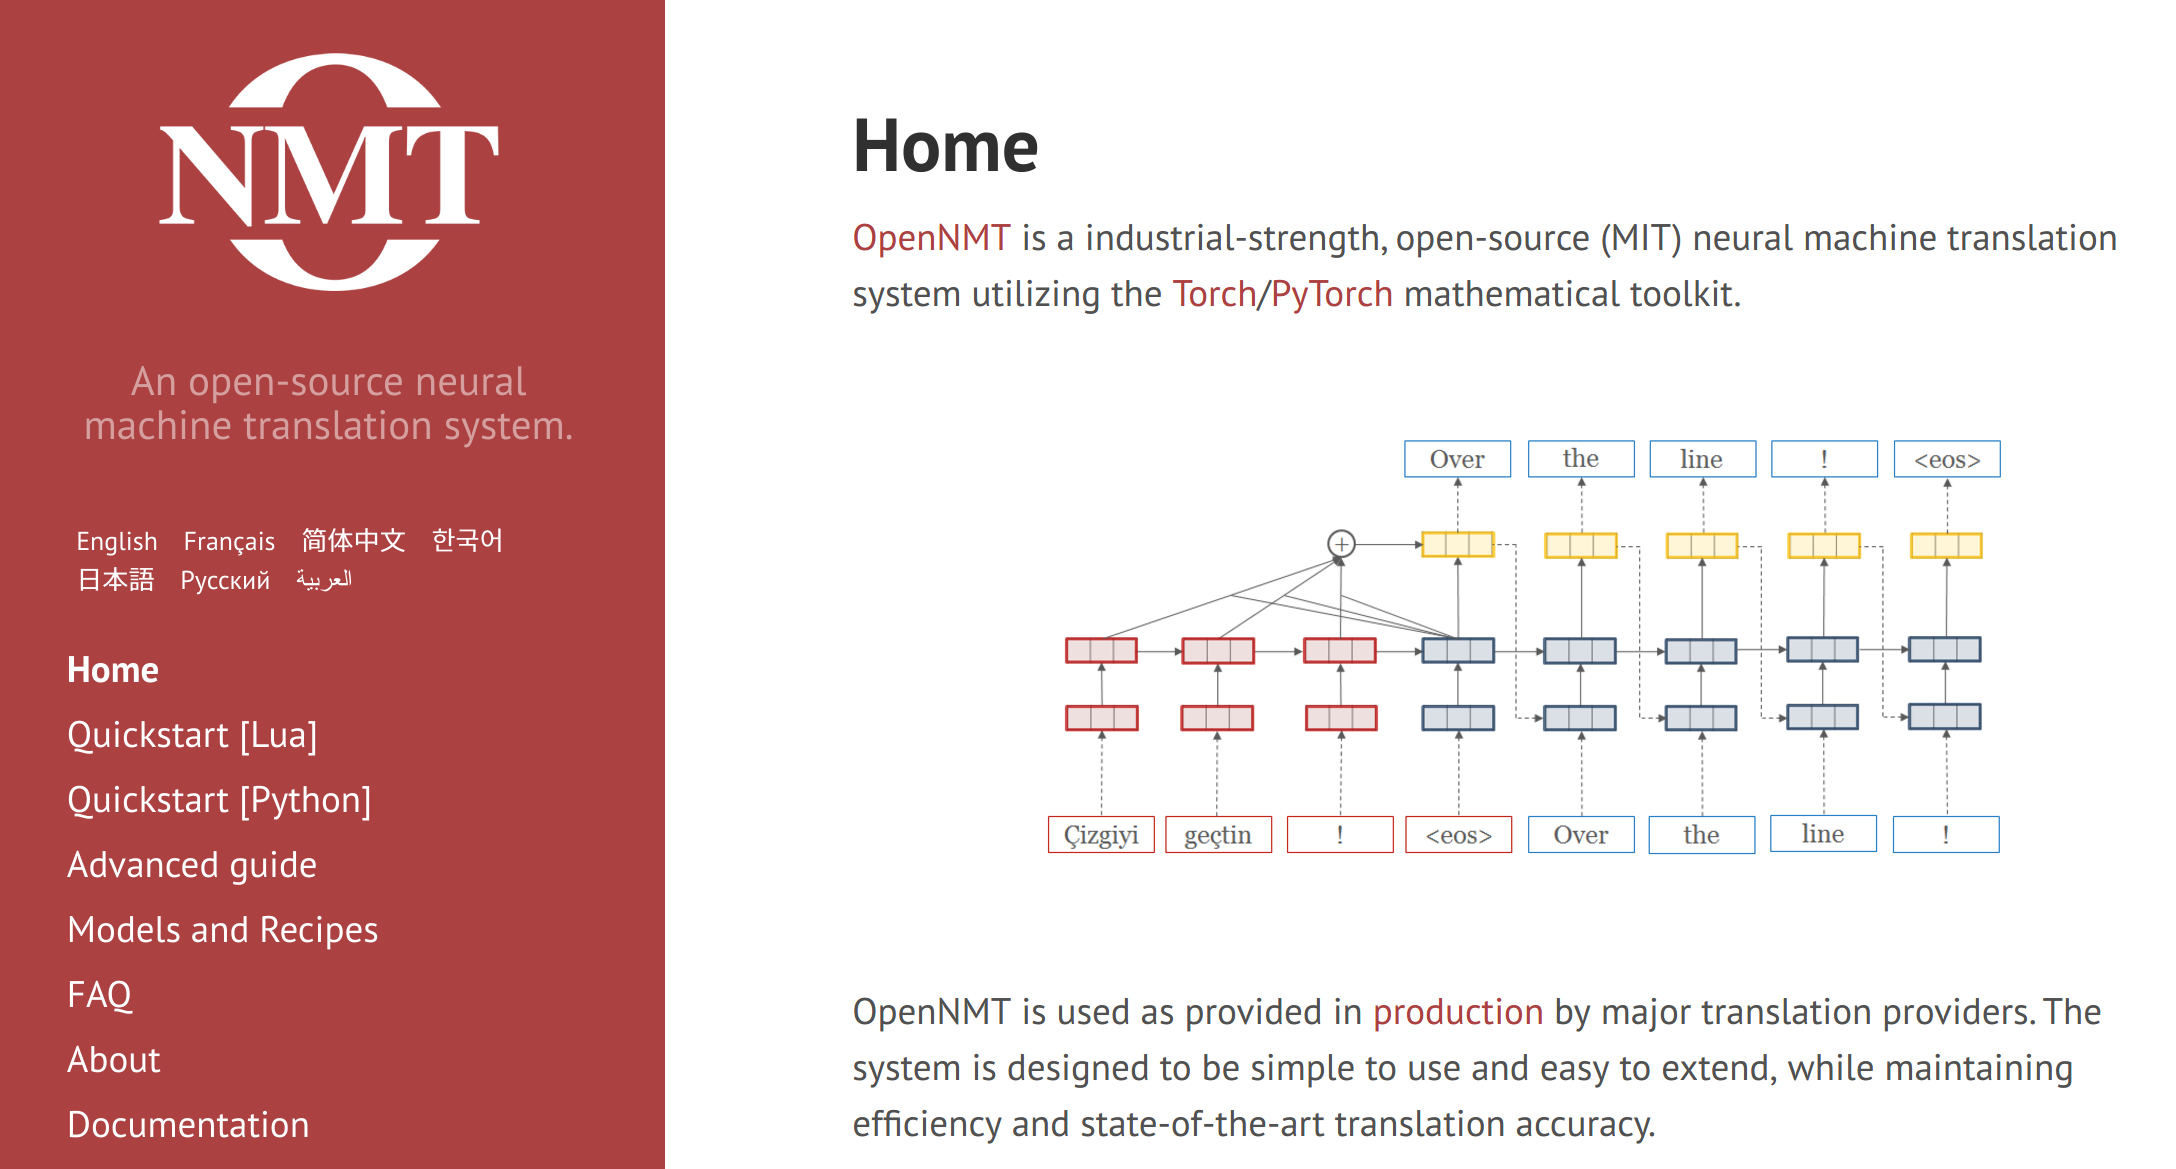
\includegraphics[width=\linewidth]{opennmt}
  \end{center}
\end{frame}

% \begin{frame}{Harvard NLP Deep Learning Research}{}
%   % Picture
%   % \research{\cite{Deng2016}}

%   \begin{center}
%     \scalebox{2}{
%   \begin{tikzpicture}

%     \node<1> at (10mm, 15mm){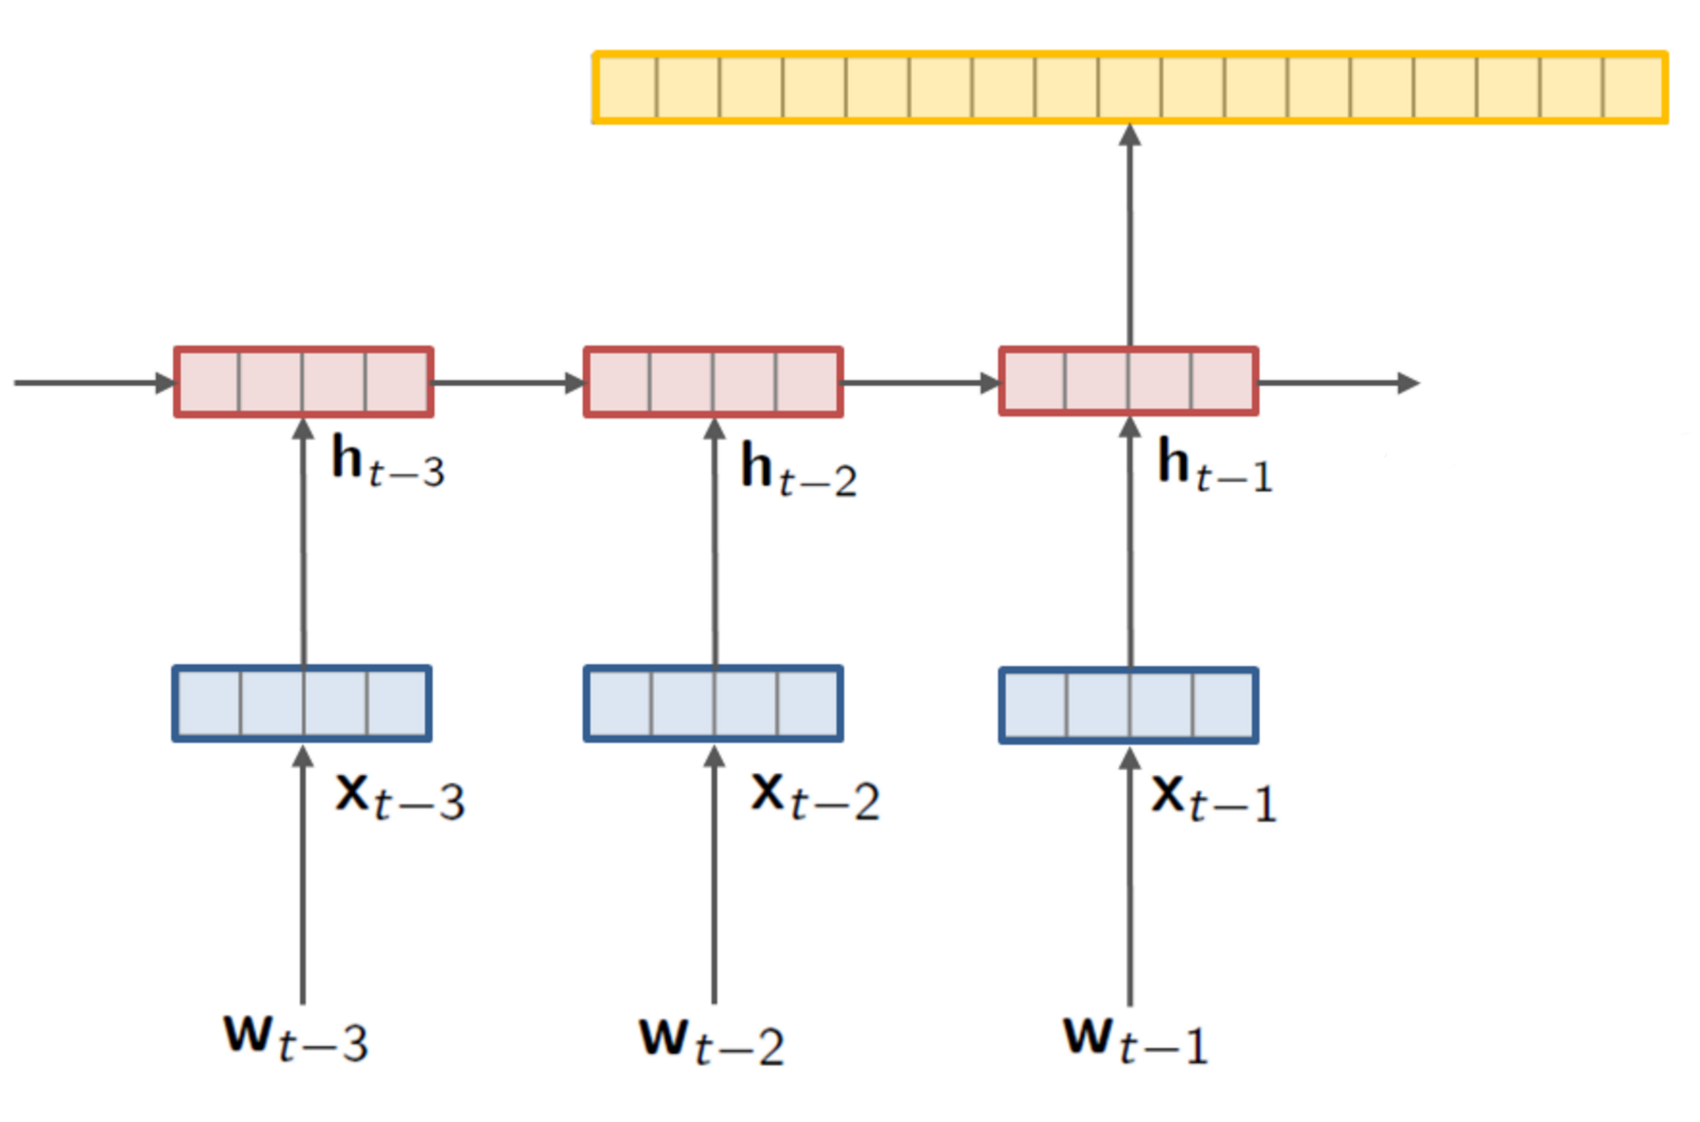
\includegraphics[width=3.4cm]{rnnlm6}};

%     \node[draw,  thick, rounded corners, scale=0.5] (ana) at (-15mm, 15mm) {Analysis};
%     \node[draw,  thick, rounded corners,scale=0.5] (meth) at (0mm, 30mm) {\ Methods\phantom{p}};
%     \node[draw,  thick, rounded corners,scale=0.5] (app) at (25mm, 30mm) {Applications};
%     % \node<2>[draw,  fill=yellow, thick, rounded corners,scale=0.5] (app) at (25mm, 30mm) {Applications};
%     % \node<2>[scale=0.5, text width=50mm] at (12mm, 15mm) {\small \centering Translation, \\  Summary,  \\ Data-to-Text,  \\ Diagram-to-Text,  \\ $\vdots$};

%     \node[draw, thick, rounded corners, scale=0.5] (und) at (35mm, 15mm) {Understanding};
%     \node[draw, thick, rounded corners, scale=0.5] (dep) at (25mm, 0mm){Scaling};

%     \node[draw,  thick, rounded corners,scale=0.5] (imp) at (0, 0) {Open-Source};

%     \draw (ana) -- (meth) --(app) -- (und) -- (dep) -- (imp) -- (ana);

%   \end{tikzpicture}
% }
%   \end{center}

% \end{frame}


\begin{frame}{Research Overview}{}
  % Pictured

  \vspace{-1cm}

  \begin{center}
  \begin{tikzpicture}

    \node at (10mm, 15mm) {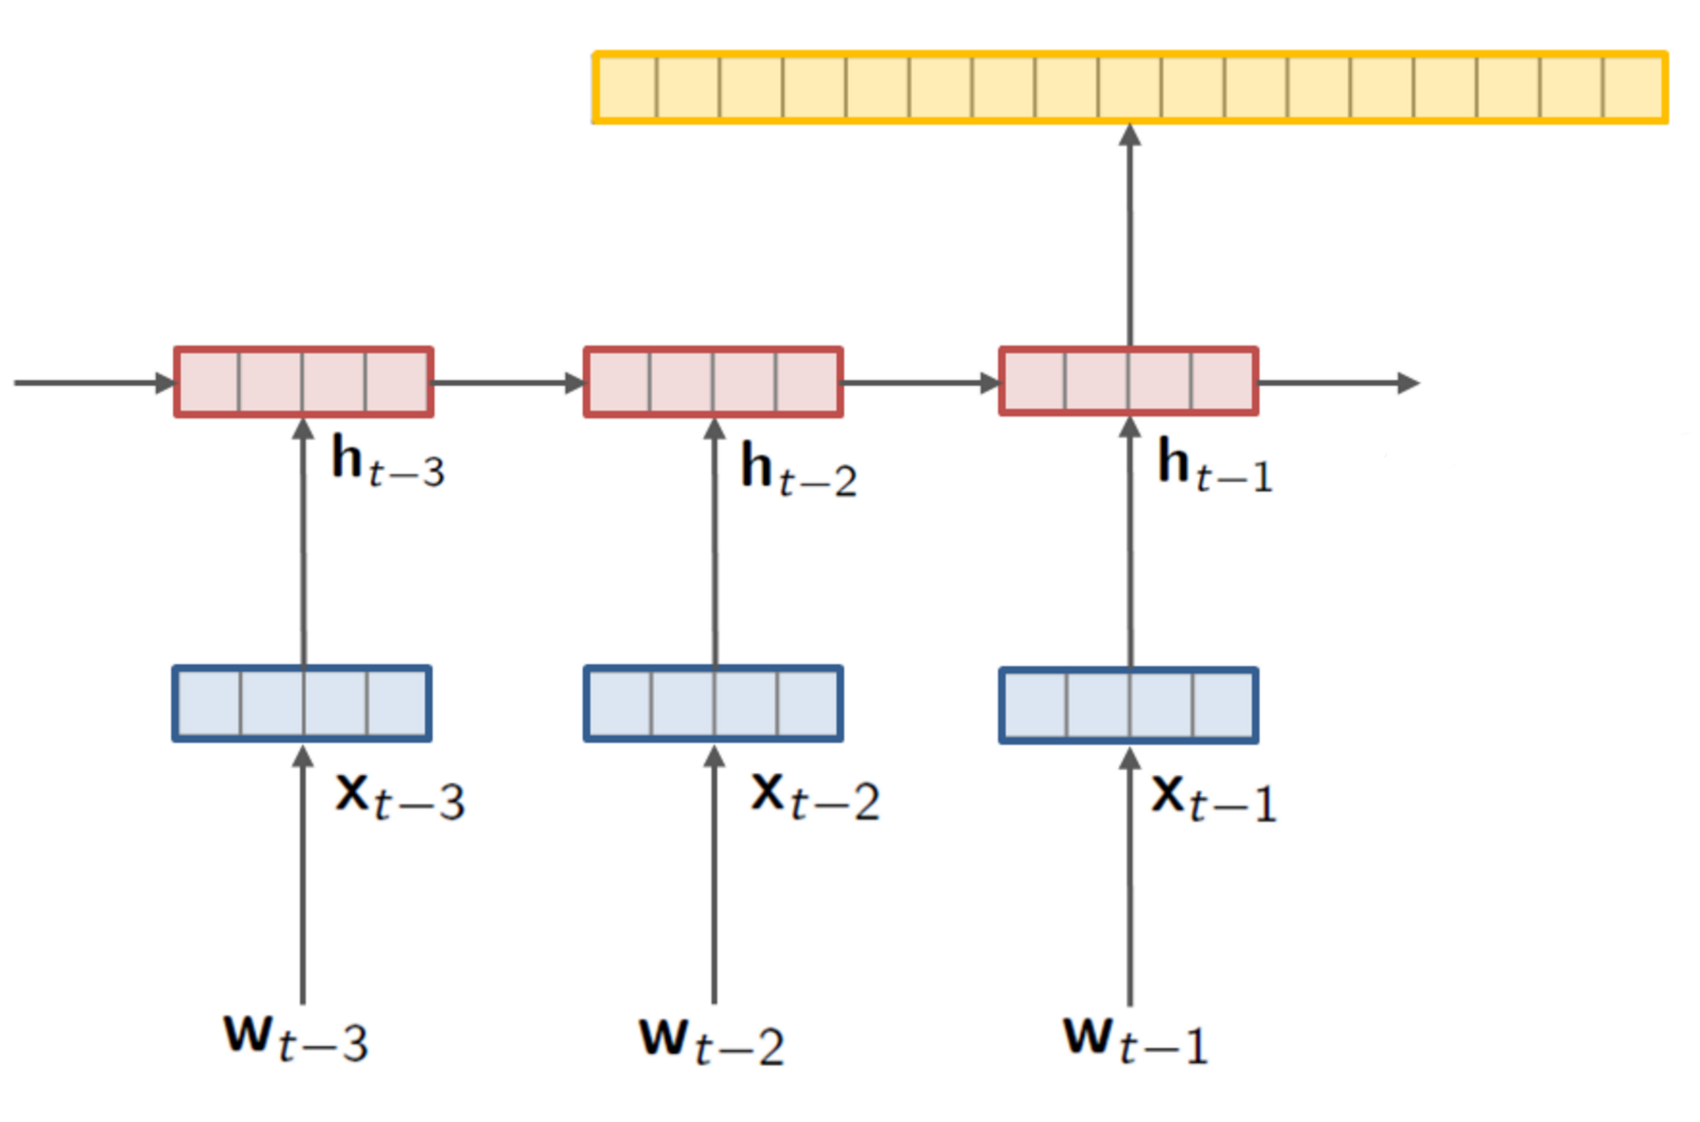
\includegraphics[width=2cm]{rnnlm6}};


    \node[rounded corners, draw] (ana) at (-15mm, 15mm) {Analysis};

    \visible{
    \node at (-40mm, 15mm) [text width=30mm]{ \centering
      \baselineskip=-5pt  \scriptsize
      \structure{
      \citet{Strobelt2016}}
    \structure{
      \citet{strobelt2019s}}
      \citet{DBLP:conf/emnlp/WisemanSR17}
      \par
      };
    }

    \node[rounded corners, draw] (meth) at (0mm, 30mm) {\ Methods\phantom{p}};

    \visible{
    \node at (-10mm, 35mm) [anchor=south, text width=30mm] { \centering

      \baselineskip=-5pt \scriptsize
      \citet{Kim2016} \ \
      \textcolor{redpurple}{\cite{DBLP:journals/corr/KimDHR17}}\ \
      \textbf{\cite{EMNLP2017}}
      \par
      };
    }
    \node[rounded corners, draw] (app) at (25mm, 30mm) {Applications};

\visible{

    \node at (35mm, 35mm) [anchor=south, text width=30mm]{ \centering
      \baselineskip=-5pt \scriptsize
      \citet{Rush2015}
      \textcolor{redpurple}{\citet{Deng2016}}
      \citet{Schmaltz2016}
      \par
      };
}

    \node[rounded corners, draw] (und) at (35mm, 15mm) {Understanding};

\visible{
    \node at (65mm, 15mm) [text width=30mm]{ \centering
      \baselineskip=-5pt \scriptsize
      \textbf{\citet{wiseman2018learning}}
      \textcolor{redpurple}{\citet{deng2018latent}}\ \ \
      \textcolor{redpurple}{\citet{DBLP:journals/corr/abs-1802-02550}}
      \par
      };
}

    \node[rounded corners, draw] (dep) at (25mm, 0mm){Scaling};

\visible{
    \node at (35mm, -10mm) [text width=30mm] { \centering
            \baselineskip=-5pt \scriptsize
            \citet{Kim2016a}
            \citet{senellart2018opennmt}
            \textcolor{redpurple}{\citet{reagen2017weightless}}
            \par
      };
}
    \node at (75mm, -5mm) [draw, text width=35mm] {\centering
            \baselineskip=-5pt \scriptsize
            Natural Lang. Processing \\
            \textcolor{redpurple}{Machine Learning} \\
            \structure{Visualization}
            \par
      };


    \node[rounded corners, draw] (imp) at (0, 0) {Open-Source};
\visible{
      \node at (-10mm, -10mm) [text width=30mm]{ \centering
        \baselineskip=-5pt \scriptsize
        \citet{DBLP:conf/acl/KleinKDSR17} \ \
        \citet{senellart2018opennmt} \ \
        \citet{rush2018annotated}
        \par
      };
}

    \draw (ana) -- (meth) --(app) -- (und) -- (dep) -- (imp) -- (ana);

  \end{tikzpicture}
  \end{center}
\end{frame}



% \begin{frame}{Recurrent Neural Network 2 - Seq2Seq + Attention}{ $f(y_{1:T}, x_{1:T}; \theta)$}
%   \vspace{-0.3cm}

%   \begin{center}
%     \multiinclude[format=png,start=1,end=10,graphics={height=0.8\textheight, trim=0.5cm 0.5cm 0.5cm
%     0.5cm, clip}]{figs/nmt-attn}
%   \end{center}
% \end{frame}

% \begin{frame}{Attention Math}

%   \textcolor{blue}{Encoder}:
%   \[{\mathbf{h}^{x}_s \gets \RNN(\mathbf{h}^{x}_{s-1}, x_s)} \]


%   \textcolor{orange}{Attention (Dynamic Context)}
%   \[\alpha \gets  \softmax(   [\mathbf{h}^{x}_1 ; \ldots; \mathbf{h}^{x}_S]^\top \mathbf{h}_{t} ) \ \ \ \
%   {\mathbf{c}} \gets \sum_{s =1}^S \alpha_s \mathbf{h}_s^{x}  \]

% \vspace{-0.3cm}

%   \begin{center}
%     \includegraphics<1>[height=0.4\textheight, trim=0.5cm 0.5cm 0.5cm
%     1.0cm, clip]{nmt-attn-5}
%   \end{center}
%   \pause
%   \vspace{-0.5cm}


%   \textcolor{red}{Decoder}:
%   \[{\mathbf{h}_t \gets \RNN(\mathbf{h}_{t-1}, y_t)} \]

%   Prediction:
%   \[ p(y_{t+1}\  |\  y_{1:t}, x) = \softmax( \mathbf{W} [\mathbf{h}_t; \mathbf{c}]) \]

% \end{frame}


% \begin{frame}{How does attention control what is said? }

%   \textcolor{orange}{Attention (Dynamic Context)}
%   \[\alpha \gets  \softmax(   [\mathbf{h}^{x}_1 ; \ldots; \mathbf{h}^{x}_S]^\top \mathbf{h}_{t} ) \ \ \ \
%   {\mathbf{c}} \gets \sum_{s =1}^S \alpha_s \mathbf{h}_s^{x}  \]


% \begin{itemize}
% \item Can we use this to control the output of the system?
%   \air

% \item Can we examine how errors enter into translation?

% \end{itemize}
% \end{frame}


% \begin{frame}{Seq2SeqVis}
%   \research{\citet{strobelt2019s} w/ IBM}
%   \vspace{-0.25cm}

%   \begin{center}
%     \movie[width=\textwidth, height=0.85\textheight, poster, showcontrols]{Temporary}{videos/seq2seq.mp4}
%   \end{center}
% \end{frame}
